\section{Przypadek Testowy 1 - Tabu Search - warianty tsp vs atsp}
  \subsection{Cel:}
    W tej części zostaną ze sobą porównane PRD rozwiązania algorytmu Tabu Search dla przypadków symetrycznych oraz asymetrycznych.
    \subsection{Założenia:}
    Do badania tego przypadku zostały wykorzystane grafy z list atsp oraz tsp. Dodatkowo liczba iteracji jest stała, równa 1000, maksymalna długość listy tabu równa 7, maksymalna liczba iteracji bez poprawy równa 10 oraz liczba sąsiadów równa 10\% wszystkich węzłów w grafie (zaokrąglona w dół).
  \subsection{Wyniki: }
  Ze względu na czytelność wszystkie wyniki są załączone w pliku \textbf(out\_test\_1\_tsp.csv) oraz \textbf(out\_test\_1\_atsp.csv).
  \subsection{Wykresy: }
    \begin{figure}[H]
      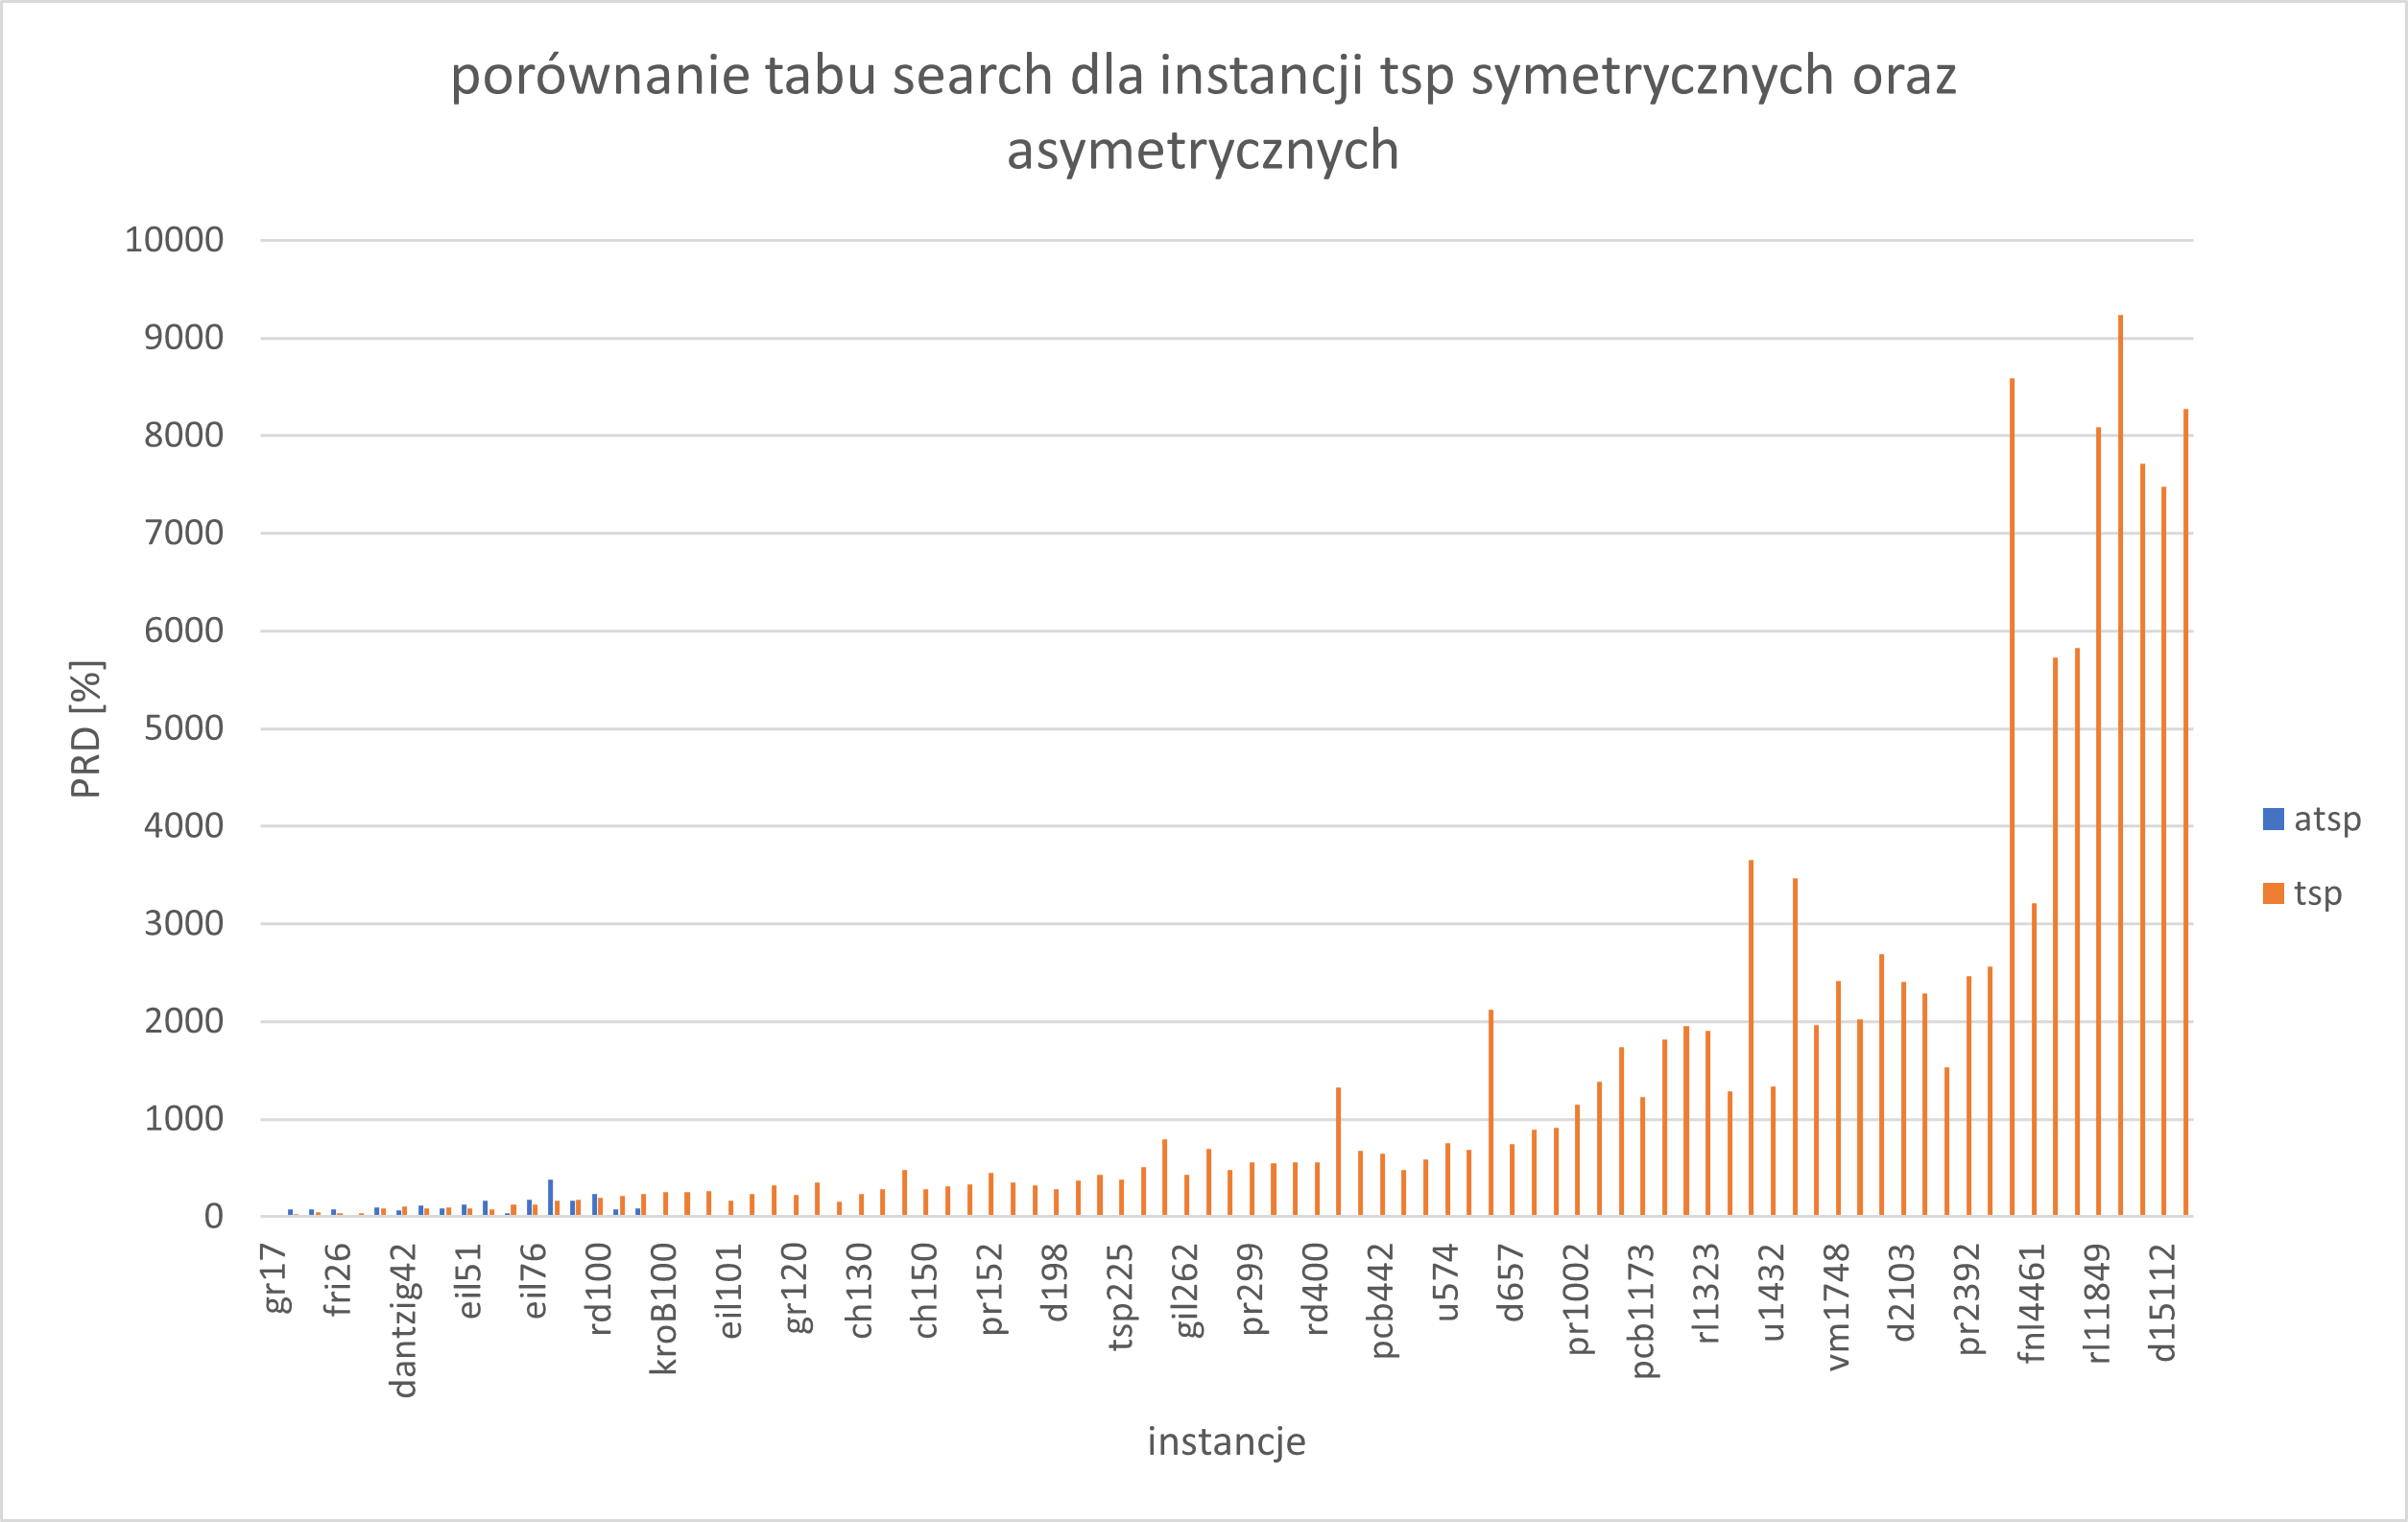
\includegraphics[scale=0.75]{chart_test1_1.png}
      \centering
      \caption{Porównanie PRD dla instancji symetrycznych oraz asymetrycznych}
    \end{figure}
    \begin{figure}[H]
      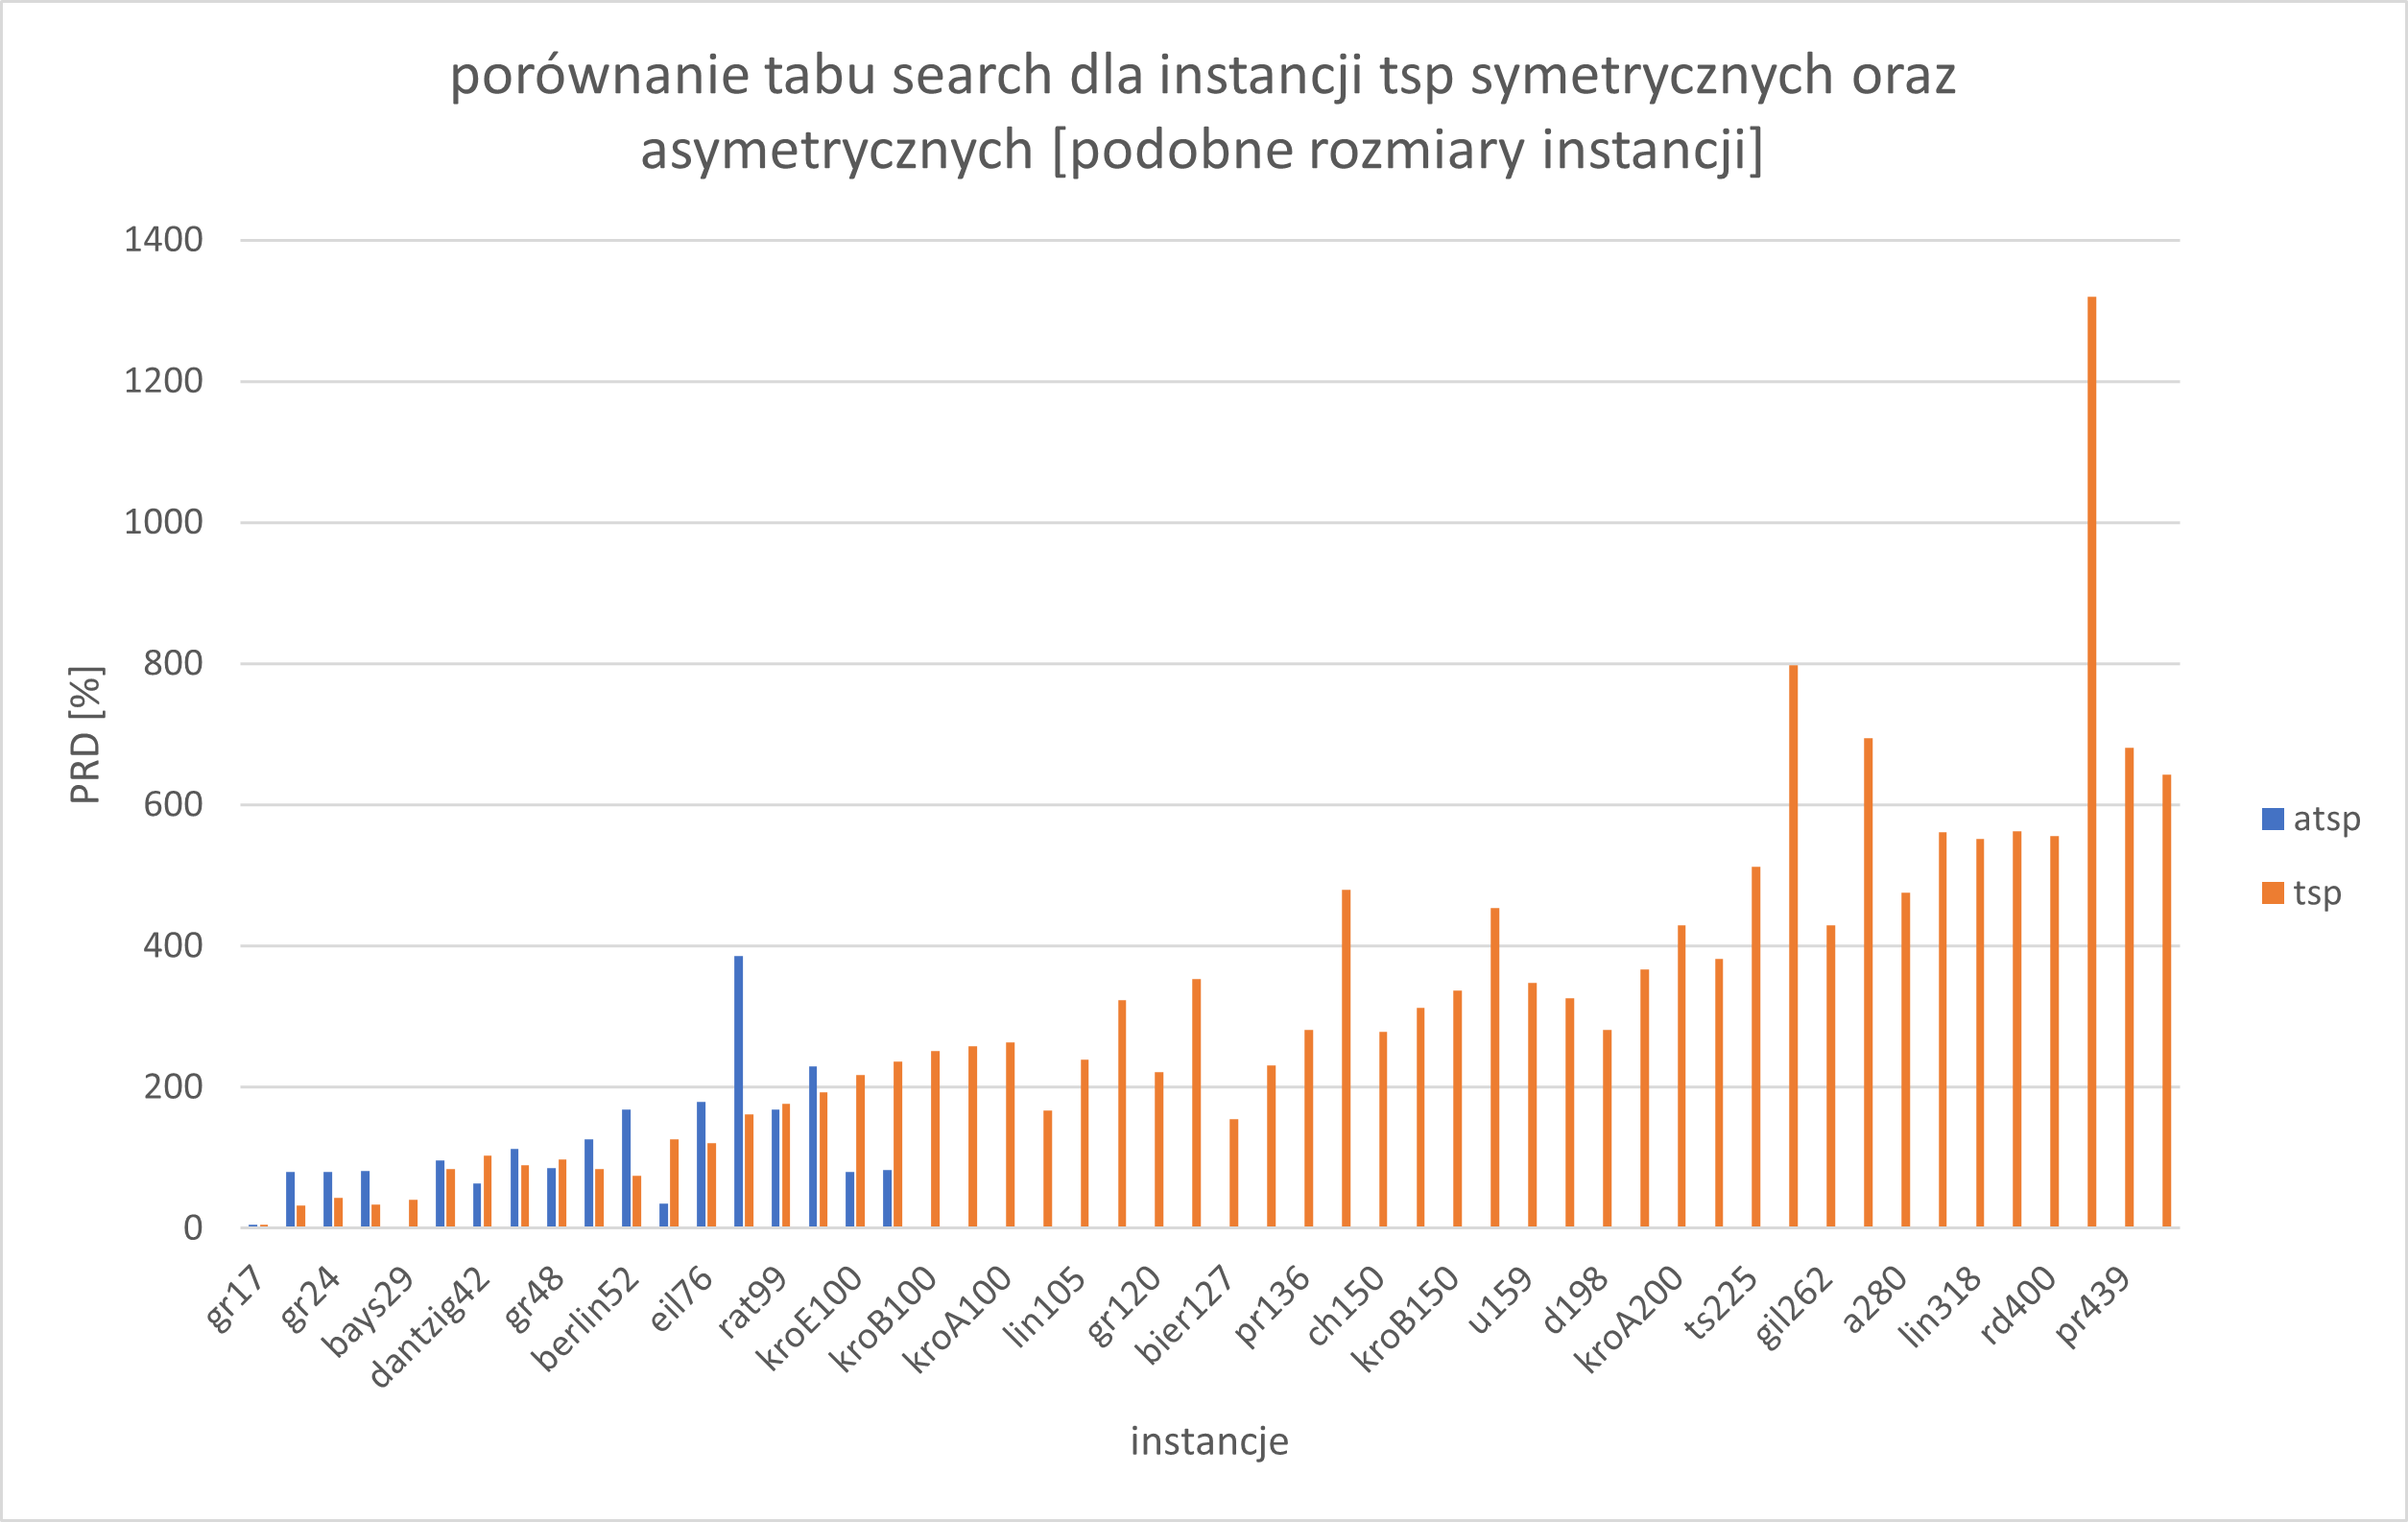
\includegraphics[scale=0.75]{chart_test1_2.png}
      \centering
      \caption{Porównanie PRD dla instancji symetrycznych oraz asymetrycznych podobnych rozmiarów}
    \end{figure}
    \begin{figure}[H]
      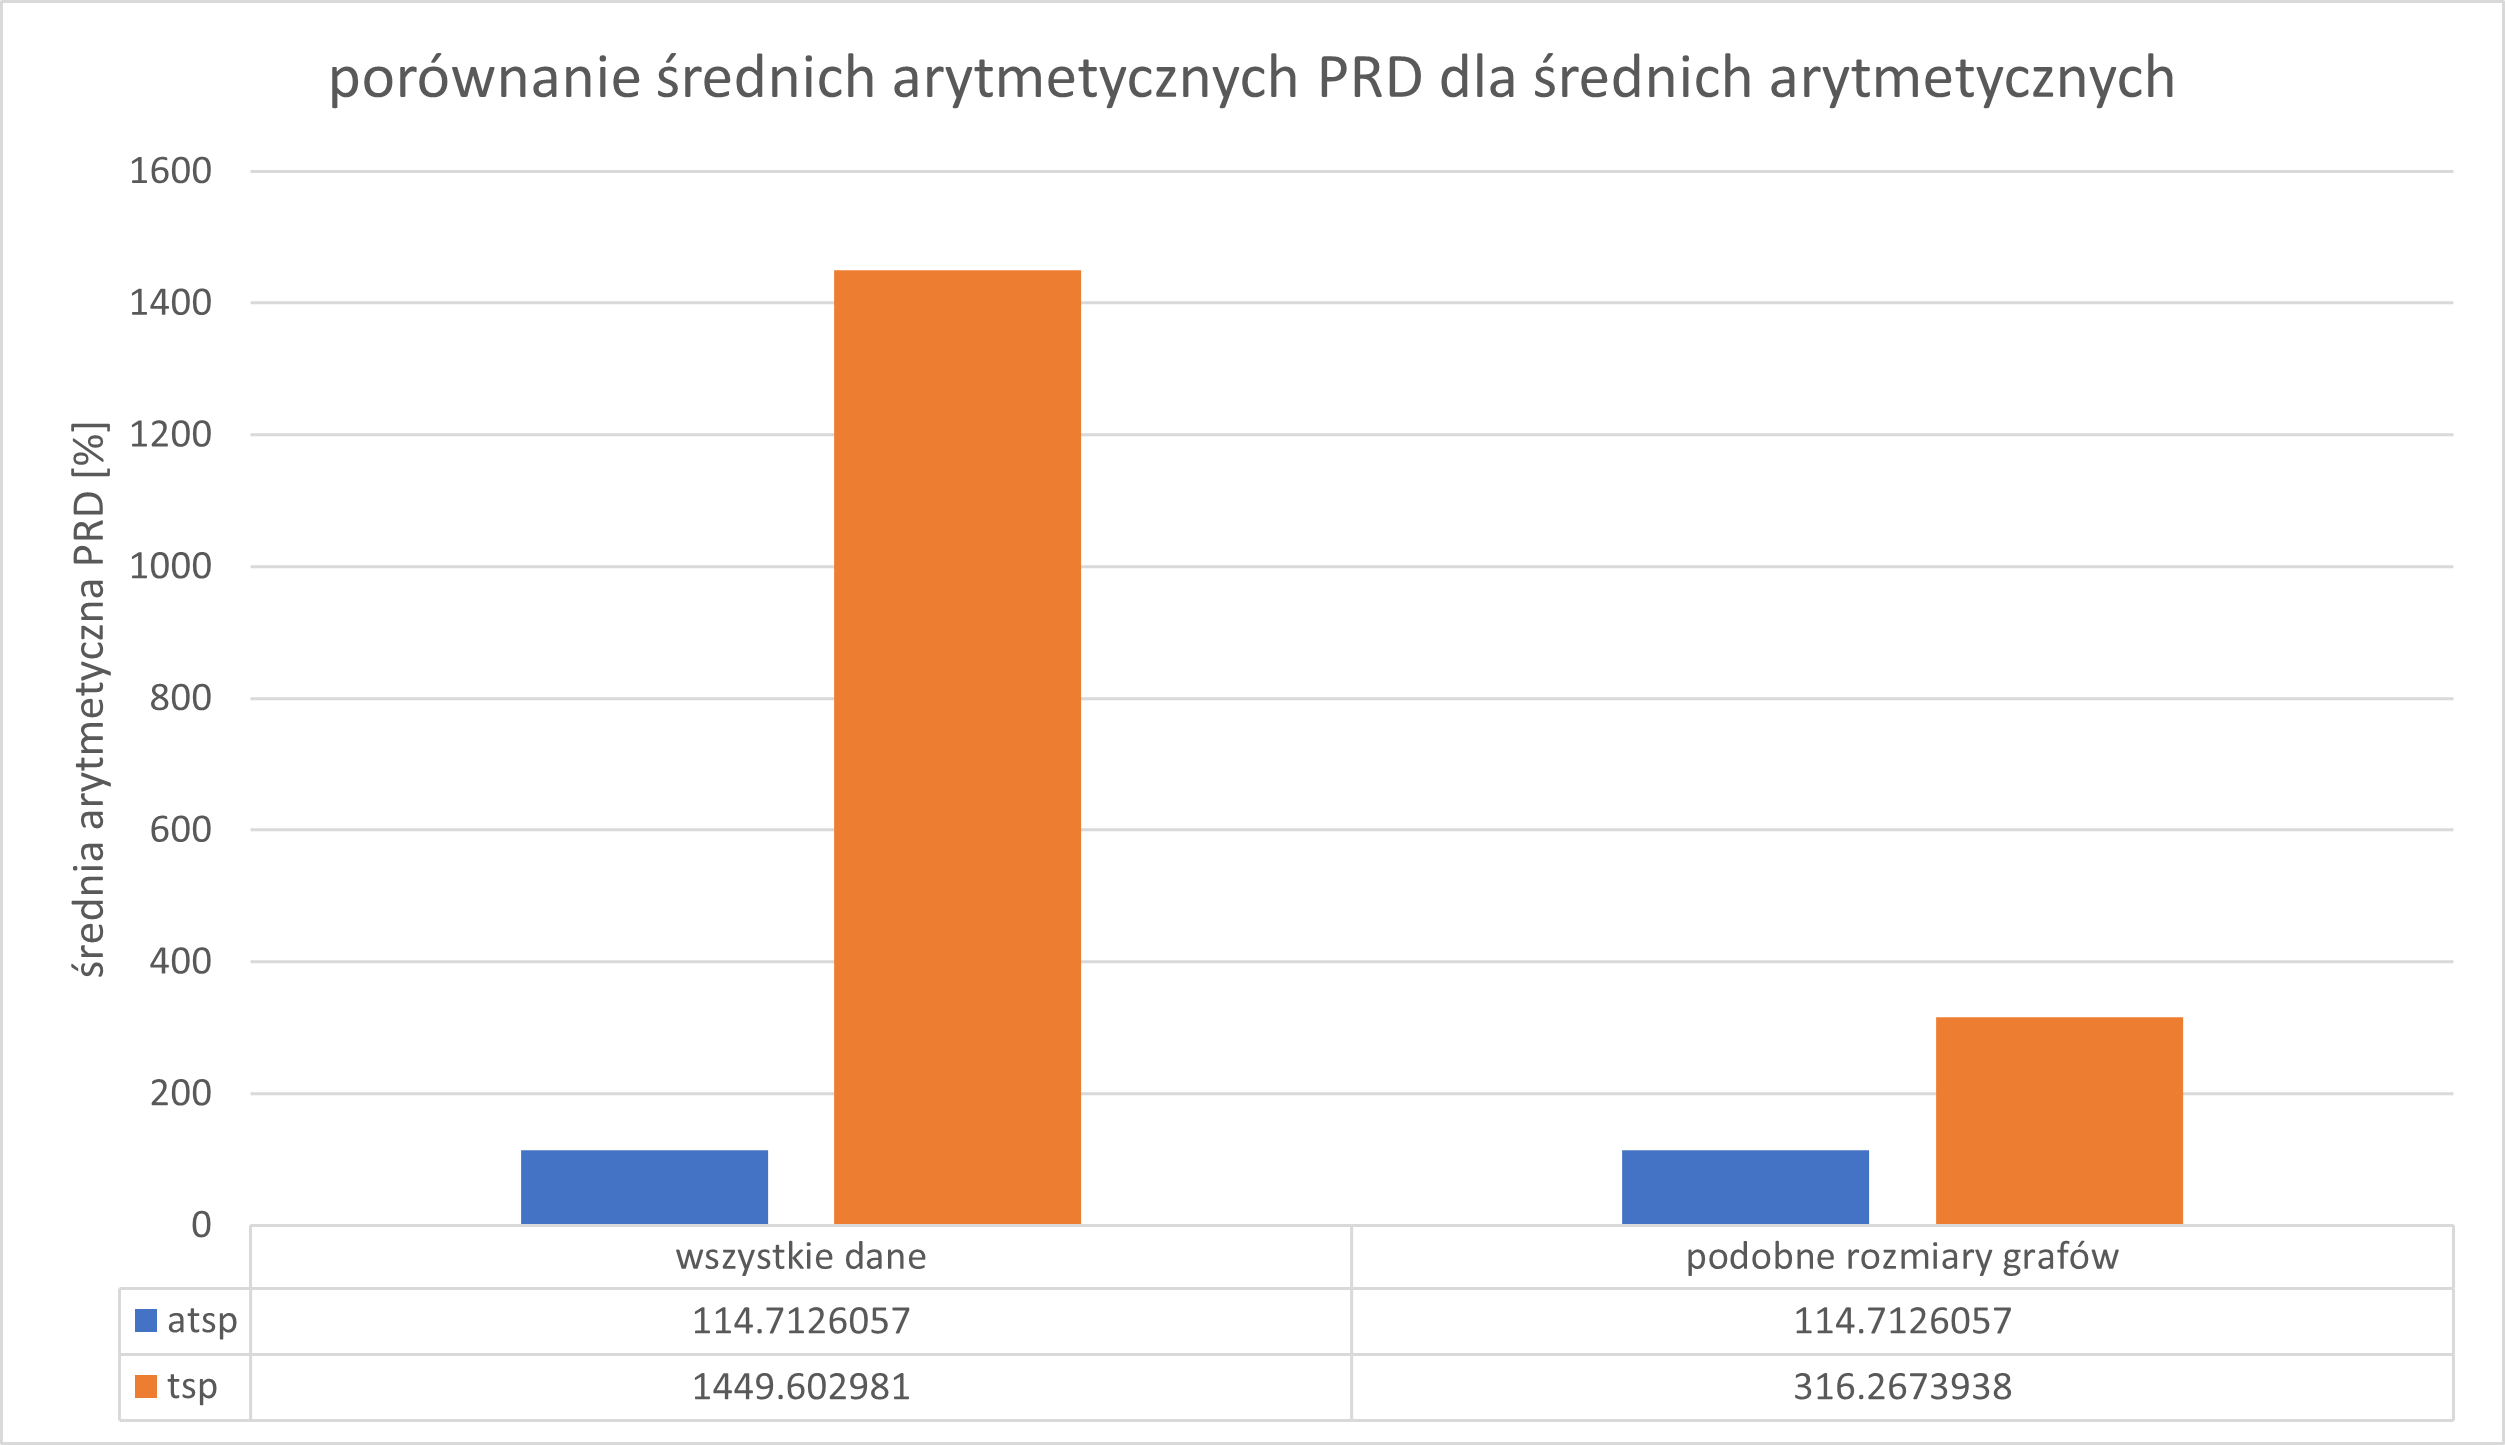
\includegraphics[scale=0.75]{chart_test1_3.png}
      \centering
      \caption{Średnie PRD dla instancji symetrycznych oraz asymetrycznych}
    \end{figure}

  \subsection{Wnioski: }
    Zauważmy, że dla danych asymetrycznych oraz zadanych parametrów algorytm średnio lepiej poradził sobie z instancjami asymetrycznymi. Widoczne jest również, że wraz ze wzrostem wielkości grafu oraz stałą liczbą iteracji algorytm radzi sobie coraz gorzej.

